\entete{FOD}{12 f\'evrier 2014}

~\\Voici une partie de la base de donn\'ees utilis\'ee pour g\'erer un site de ventes en ligne. La soci\'et\'e dispose de plusieurs entrep\^ots, un par d\'epartement (de France).

\begin{tabular}{l}
\texttt{PRODUIT}(\underline{id}, nom, prix, cat\'egorie, fournisseur, marque)\\
\texttt{CLIENT}(\underline{id}, nom, pr\'enom, adresse, d\'epartement)\\
\texttt{COMMANDE}(\underline{id\_client, id\_produit}, date, quantit\'e)\\
\texttt{STOCK}(\underline{id\_produit, d\'epartement}, stock)\\
\end{tabular}


\section{Alg\`ebre relationnelle et SQL (10 points)}

\begin{enumerate}
\item Identifiez les cl\'es primaires et \'etrang\`eres pour la table STOCK. (0.5 points)
\begin{correction}
\begin{lstlisting}
Cles primaire : (id_produit, departement)
Cles etrangeres :  id_produit->PRODUIT(id)
\end{lstlisting}
\end{correction}

\item Donnez la commande SQL pour cr\'eer la table STOCK. (0.5 points)
\begin{correction}
\begin{lstlisting}
CREATE TABLE STOCK(
	id_produit INTEGER,
	departements VARCHAR(20),
	quantite_en_stock,
	CONSTRAINT pk_stock PRIMARY_KEY (id_produit, departement),
	CONSTRAINT fk_stock FOREIGN_KEY (id_produit)
		REFERENCES PRODUIT(id))
\end{lstlisting}
\end{correction}


\item Donnez les noms et pr\'enoms des clients qui ach\`etent des produits de la marque 'Apple'  (Alg\`ebre et SQL, 1 point)
\begin{correction}
\begin{lstlisting}
SELECT nom, prenom FROM COMMANDE com, CLIENT cl, PRODUIT p
WHERE com.id_client = cl.id AND
	com.id_produit = p.id AND
	p.marque = 'Apple';
\end{lstlisting}
\end{correction}

\item Donner les noms et pr\'enoms des clients dont une commande ne peut \^etre satisfaites (la quantit\'e demand\'ee d\'epasse le stock disponible dans leur d\'epartement). (Alg\`ebre et SQL, 2 points)
\begin{correction}
\begin{lstlisting}
SELECT nom, prenom 
FROM CLIENT cl, COMMANDE com
WHERE cl.id = com.id_client AND
	quantite  > 
		(SELECT quantite_en_stock  
		FROM STOCK s WHERE s.id_produit = com.id_produit 
		AND s.departement = cl.departement)
\end{lstlisting}
\end{correction}

\item Donnez les noms des produits qui ne sont pas disponibles dans aucun entrep\^ot (SQL seulement, 2 points)
\begin{correction}
\begin{lstlisting}
SELECT p.nom FROM PRODUIT p, COMMANDE c
WHERE c.id_produit = p.id AND 
	c.id_produit NOT IN (SELECT DISTINCT id_produit FROM STOCK);
\end{lstlisting}
\end{correction}

\item Donner les nom et pr\'enoms des clients ayant command\'e plus de 10 agendas aujourd'hui. (SQL seulement, 2 points)
\begin{correction}
\begin{lstlisting}
SELECT nom, prenom FROM  COMMANDE com, CLIENT cl, PRODUIT p
WHERE com.id_client = cl.id AND 
	com.id_produit = p.id AND p.nom = 'Agenda'
GROUP BY id_client
HAVING SUM(quantite) > 10�;
\end{lstlisting}
\end{correction}

\item Donnez les noms et pr\'enoms des clients qui ont achet\'e un des produits les plus chers de la marque 'Samsung'. Attention ! : plusieurs produits peuvent avoir le m\^eme prix. (SQL seulement, 2 points)
\begin{correction}
\begin{lstlisting}
SELECT DISTINCT nom, prenom
FROM COMMANDE com, CLIENT cl, PRODUIT p
WHERE marque = 'Samsung' AND
	id_produit = p.id AND id_client = cl.id AND
	p.id_produit IN 
		(SELECT MAX(prix) FROM PRODUIT 
		WHERE marque = 'Samsung')
\end{lstlisting}
\end{correction}
\end{enumerate}

\section{Indexation (3 points)}

\begin{enumerate}
  \item On souhaite créer une index B+Tree d'ordre 2 sur l'attribut {\tt
  COMMANDE.date}. Construire l'arbre correspondant à l'ensemble de valeurs
  ci-dessous, en respectant l'ordre d'arrivée. Donner les étapes de construction
  intermédiaires importantes (celles qui produisent un changement de la
  structure de l'arbre). (2 points)\\
\texttt{2013-12-15, 2013-12-23, 2013-12-20, 2014-01-13, 2013-12-18,\\ 2013-12-21, 2014-01-20, 2013-12-21, 2014-01-05, 2014-02-08,\\ 2014-01-25}
\begin{correction}
\begin{figure}[h!]
\begin{center}
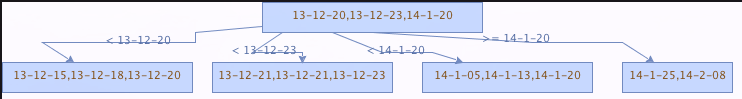
\epsfig{file=Fig/2014-02_btree.png, width=\textwidth}
\end{center}
\end{figure}
\end{correction}

  \item On souhaite r�cup�rer toutes les commandes pass�es depuis le '01/01/2014'. Si un noeud de l'index est une page sur le disque, combien de pages de l'index doivent �tre lues pour r�pondre � cette requ�te ? (1 point)
\begin{correction}
Il faut chercher la plus grande valeur avant le '01/01/2014' et parcourir les pages � partir du noeud trouv� jusqu'� la derni�re feuille.
Ainsi, on va trouver le noeud contenant '2013-12-23', puis parcourir les deux autres feuilles. Ce qui nous fait au total 4 pages d'index (1xracine, 1xrecherche, 2xparcours).
\end{correction}
\end{enumerate}


\section{Optimisation (4 points)}

\begin{enumerate}
 \item (1 point) Pour la requ�te ci-dessous, dire ce quelle produit comme r�sultat.
\begin{lstlisting}
  SELECT nom
  FROM Produit P, Commande C
  WHERE P.id=C.id_produit
        AND prix > 100
        AND quantite > 10
        AND marque = 'Bricoflex';
\end{lstlisting}
\begin{correction}
Donner les noms des produits de marque Bricoflex ayant un prix sup�rieur � 100 (l'unit�), ayant une commande de plus de 10 unit�s (chaque commande).
\end{correction}
 \item (3 points) Donner un plan d'ex�cution (EXPLAIN \underline{et} arborescent) sachant qu'il existe un index sur l'attribut {\tt marque} de la table {\tt Produit}, qu'il n'y a pas d'autres index et que les deux tables sont de tailles moyennes.
Ne pas oublier d'ajouter l'emplacement des diff�rents filtres de la requ�te.
\begin{correction}
\begin{verbatim}
0  SELECT STATEMENT
1*   NESTED LOOPS
2*     TABLE ACCESS BY INDEX ROWID   Produit
3*       INDEX RANGE SCAN            IDX_Marque
4*     TABLE ACCESS FULL             Commande

(1) P.id=C.id_produit
(2) prix > 100
(3) marque = 'Bricoflex'
(4) quantite > 10
\end{verbatim}
\end{correction}
\end{enumerate}

\section{Concurrence (3 points)}

Soit l'ex\'ecution concurrente suivante de trois transactions dans un SGBD.

\textbf{H:} $r_1[x] r_2[x] r_1[y] w_2[y] r_3[x] w_1[x] r_3[y] c_1 c_2 a_3$

\begin{enumerate}
   \item Existe-t-il une ``lecture sale''~? Pourquoi faut-il \'eviter
   ce type de lecture (expliquer les effets possibles)\,? (1~point)

     \item Quelle est l'ex\'ecution obtenue par verrouillage \`a deux phases
   \`a partir de $H$? On consid\`ere que le relachement des verrous d'une
   transaction se fait au Commit et qu'\`a ce moment on ex\'ecute en priorit\'e les op\'erations bloqu\'ees
      en attente de verrou, dans l'ordre de leur blocage. (2~points)
\end{enumerate}
